
\chapter{Research Design}
\label{design}


This project will assess the viability of using Gaussian Process models for spatiotemporal predictions in urban settings. Gaussian Processes have attractive properties for sparse data because a model can be interpreted as interpolating an unobserved point between known distributions. As mentioned in the literature review, spatiotemporal models have historically suffered from computational infeasibility when the amount of data as well as spatial and temporal dimensionality grows. Recent advances in Bayesian probablistic programming and implementations of Gaussian Processes that take advantage of the relative sparsity of data across spatial dimensions has reduced the computational burden of fitting these models. \par


\section{Gaussian Processes}

A Gaussian Process (GP) is a generalization of a Gaussian - also known as the Normal - distribution. A Normal distribution is defined by a scalar mean $\mu$ and variance $\sigma$ in the univariate case, and a n-length vector $\mathbf{\mu}$ with a n-by-n dimensional covariance matrix $\Sigma$ in the multivariate case. A Gaussian Process ''can be viewed as a potentially infinite-dimensional generalization of [the] Gaussian distribution'' \cite{gelman2013bayesian} , p. 501. However any finite-dimensional marginal distribution from a Gaussian Process is also Gaussian, which makes a GP suited as a prior distribution for some unknown regression function $\mathbf{\mu}(x)$ - where $x$ is a vector with arbitary but finite dimensions. A generic Gaussian Process $\mu \sim GP(m,k)$ is a series of random functions drawn from an n-dimensional normal distribution \cite{gelman2013bayesian}: \par

$$ \mu(x_1),...,\mu(x_n)) \sim N((m(x_1),...,m(x_n)),K(x_1,...,x_n)) $$

Thus a Gaussian Process is defined entirely by a mean function $m$ and covariance function/s $K$. Sums and products of GPs are also GPs, which makes it simple to combine different variations of covariance functions.

\subsection{Estimating Gaussian Processes}

While it is not necessary to go into extensive detail about the theory of Gaussian Processes for this application, it is relevant to briefly describe what part of the estimation poses a challenge for high-dimensional datasets like those found in spatiotemporal forecasting. To generate samples from a finite-dimensional realization of a GP $\mathbf{\mu} \sim N(\mathbf{m},K)$, it is necessary to calculate the Cholesky decomposition of the covariance matrix: $K=LL^\intercal$. Then it easy to generate standard Normal draws $\mathbf{u} \sim N(\mathbf(0),I)$, and shift them using $\mathbf{\mu}=\mathbf{m}+L\mathbf{u}$ \cite{rasmussen_2005}. Calculating $L$ is quite computationally demanding as $n$ rises. In practice the eigenvalues of $K$ can also decay, causing the decomposition to fail. This is solved in practice by adding a small 'jitter' term to the diagonal of $K$. Ideally the jitter term is small enough to not influence the estimates, but this has to be assessed through trial and error. \par


\section{The Log-Gaussian Cox Process}

Log-Gaussian Cox Process (LGCP) models are a further extension of a Gaussian Process with particular applicability to prediction of count data. A LGCP is hierarchical in that the data are assumed to be drawn from a Poisson likelihood with intensity parameter $\lambda$. The Poisson likelihood function has theoretical properties suitable for relatively sparse count (integer) data which makes it appealing for use in modelling frequent events that are nevertheless sparse when segmented over space and time dimensions. In turn the log of $\lambda$  is generated by a Gaussian process\cite{teng_2017}. This makes the LGCP quite flexible in inputs and dimensionality while also making model fitting generally computationally burdensome. \par

An alternative specification uses a Gaussian likelihood, which has the added appeal of making the likelihood and prior conjugate to each other and solvable in closed form. As the $\lambda$ parameter of a Poisson distribution increases the distribution converges to a Normal distribution anyway, so this model may be more applicable to situations when counts are not sparse e.g., at lower granularities of space and/or time, which was not considered in detail here.

A zero-inflated Binomial (ZIB) likelihood would be another alternative to consider for this type of modelling. As the name implies, a ZIB distribution has a higher probability density around zero and may be better suited for extremely sparse data like gridded observations with very small grid dimensions.

 The general model follows the specification and notation used by "A General Approach to Prediction and Forecasting Crime Rates with Gaussian Processes" \cite{flaxman_2014}: \par


$$\lambda(s,t) = exp((s,t))$$

$$ y_{s,t} | \lambda(s,t) \sim Poisson(exp(f(s,t))e_s) $$

The outcome count $y_{s,t}$ at location $s$ and time $t$ is generated from a Poisson distribution whose scale parameter is a the function $f(s,t)e_t$. $f(s,t)$ is a function with a Gaussian process prior, while $e_s$ is a fixed spatial expectation term $\mathbb{E}[y_s]$. The spatial expectation is a convenient way to incorporate prior information about the variable of interest. Again following Flaxman 2014, using an exponential link function gives a practical interpretation of $exp(f(s,t))$ as the relative risk function while $f(s,t)$ itself is the log-relative risk. When the log-relative risk is 0, the relative risk is 1 and the expected value of of the outcome $y(s,t)$ is just the prior spatial expectation $e_s$. Finally, every count outcome $y_{s,t}$ is assumed independent conditional on $f$, so the joint conditional likelihood of all $y$ factors as a product.

$$p(y|f) = \prod_{s,t}{ Poisson( y_{s,t}| exp(f(s,t))e_s)}$$

\subsection{f(s,t)}

$f$ is modeled as following a generic Gaussian process with a mean of zero and a covariance matrix $K$:

$$ f \sim GP(0,K) $$

Spatiotemporal elements enter the Gaussian process model through $K$, which is used to capture the relationships of interest and entirely determines the model. Since variance/covariance is additive, any variance term can be decomposed at least theoretically into arbitrarily many additive components. Purely spatial and temporal elements as well as interactions can be incorporated using different kernel functions, and different combinations of kernels may produce more accurate results. Cross-validating models with different types and combinations of kernel functions will help identify the specification with the best predictive properties. Since the cross-validation data are correlated in this model the cross-validation set will have to be drawn from spatially contigous representative subsets of the data.

\subsection{Kernels}

There are a wide variety of existing kernel functions documented for use in Gaussian process models \cite{rasmussen_2005} and it is also possible to define custom functions as long as they follow certain properties. The entirety of a GP is determined by its kernel/s, which makes them versatile and open to many different specifications. \par

An important consideration is whether the model is considered to be stationary. In spatiotemporal models the case for assuming stationarity weakens as the time-period being considered lengthens, and this should in turn affect the kernel choice. The long term model considered includes a non-stationary linear kernel component intended to capture any long-term trends:    \par

\begin{itemize}
  \item $k_t(t)$ : a temporal kernel
  \item $k_p(t)$ : a periodic kernel
  \item $k_l$: a linear kernel
\end{itemize}

The short-term models considered for this project are all stationary and loosely follow Flaxman 2014 by consisting of up to four individual kernels $k$ , where $K=\sum_{i}k_i$. The four basic kernel types were:

\begin{itemize}
  \item $k_s(s)$ : a spatial kernel
  \item $k_t(t)$ : a temporal kernel
  \item $k_p(t)$ : a periodic kernel
  \item $k_{st}(s,t)$ : a space-time interaction kernel
\end{itemize}

Radial Basis Function (RBF) and Matern family kernels are both candidates for spatial and temporal modeling. Their point of differntiaion lies in the extent to which they 'smooth' the input. The most appropriate kernel will vary based on the characteristics of the observations being modeled.

The RBF kernel - also called the squared exponential - is widely used as a default stationary kernel:

$$ k_t(t) = exp\big(- \frac{(|t-t'|)^2}{2\ell^2}\big) $$

The L1 norm $|t-t'|$ of the input determines the kernel, along with $\ell$,  a lengthscale parameter that is common to kernel functions.

The Matern family kernels are defined:

$$ k_t(t) = \frac{1}{2^{\nu - 1}\Gamma(\nu)}\big(\frac{\sqrt{2\nu}}{\ell}(|t-t'|)\big)^\nu K_{\nu}\big(\frac{\sqrt{2\nu}}{\ell}(|t-t'|)\big)$$

The parameter $\nu$ determines the degree of smoothness and the kernel converges to a Gaussian kernel as $\nu$ goes to $\inf$. Typical values of $\nu$ are fractions,with $\nu=\frac{1}{2}$ or $\frac{3}{2}$ being quite common. The name of a specific kernel is often expressed by referencing the parameter value, so in this paper a 'Matern32'  refers to a Matern kernel with $\nu=\frac{3}{2}$. Figure \ref{kernel_examples} shows a comparison of the degree of smoothing a RBF,Matern12, and Matern32 kernel have on the same multivariate random input:

\begin{figure}[h!]
  \centering
  \caption{A comparison of RBF with Matern family kernels.}
  \label{kernel_examples}
  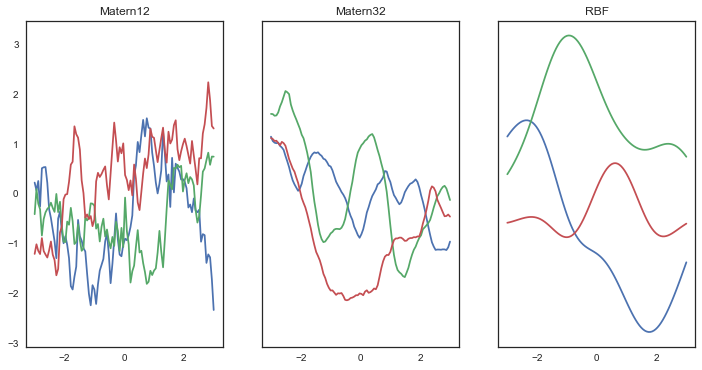
\includegraphics[width = 0.8\textwidth]{kernel_examples}
\end{figure}


The periodic is another class of stationary kernel. The variant used in this project follows MacKay 1998  \cite{mackay1998introduction}:

$$ k_p(t) = exp \bigg[ - \frac{1}{2}\sigma_i \big(\frac{sin(\frac{\pi}{\Delta}(t_i - t_i'))}{\ell} \big)^2 \bigg] $$

$\Delta$ is a periodicity paramter that can either be fit or set to a fixed anticipated value such as 52 for annual weekly data. $\ell$ is again the lengthscale parameter.\par


\subsection{Priors}

Gelman 2006 suggests using a student-t prior distribution restricted to be positive (a 'half-t') as a prior for variance parameters in hierarchical models \cite{gelman_2006}. Since variance is always positive it is acceptable and desirable to restrict the prior distribution to be non-negative as well. Flaxman 2014 used a standard student-t prior with 4 degrees of freedom on all parameters (not just variance). Both standard Normal $N \sim (0,1)$ and Student-T priors were considered here. The normal prior has less probability mass in its tails than the Student-t but is otherwise a close substitute. The Normal prior did sometimes lead to the optimization algorithm failing to find a credible set of parameter estimates, while the Student-T with degrees of freedom between 2 and 10 performed better. Increasing the variance on the prior distributions was another way to lower the probability of the optimizer failing, but it also led to dramatically increased runtimes in some cases.

\section{Methods for fitting LGCPs}

Solutions to the computational challenges in fitting LGCPs have advanced rapidly over the past five years. As mentioned earlier, the computational bottleneck for Gaussian Process models is the the n-by-n covariance matrix, which requires an $O(n^3)$ computation. Fitting a GP model as $n$ grows beyond a few thousand points is quite challenging \cite{gelman2013bayesian}. \par

 As recently as 2012 the best methods for fitting LGCP models involved variations of the Metropolis-Hastings sampling algorithm which were considered to be slow and highly inefficient in generating acceptable draws from the posterior distribution of the model \cite{murray_2012}. Advances in statistical computing have opened the door for several new model fitting methods, each with their own advantages and drawbacks.

\subsection{Variational Inference}

Variational Inference (VI) methods attempt to recover parameter estimates for a posterior distribution of interest by specifying a more tractable family of distributions and optimizing the resulting approximation using closed-form or computational methods. Usually the family of approximating distributions is denoted $Q$, and the optimization seeks to minimize the Kullback-Leiber divergence $KL[(\theta), p(\theta|y)]$ between $q(\theta)$ and the true posterior $p(\theta|y)$. \par

In the case of the LGCP with Poisson likelihood there is no direct closed-form solution because an intractable integral is involved. VI methods have in the past been limited by needing to make simplifying assumptions about the approximating distributions. Usually VI makes the 'mean-field' assumption (borrowed from physics), that the posterior can be approximated by the product of some number of existing distributions: $q(\theta_1,...,\theta_n)= \prod_j{q_j(\theta_j)}$. The mean-field assumption is especially unsuited for high-dimensional models like a Gaussian Process, but Tran and Blei characterize a Variational Gaussian Process method that avoids the assumption \cite{tran_2015}. GPflow - the package used for this project - uses the Variational Gaussian  for fitting \cite{GPflow2017}.\par

The major drawback of variational methods is there are no theoretical justifications for the accuracy of estimates produced because it is unclear and often unknowable how close the optimized approximation is to the true posterior distribution, where the $KL$ divergence term is a unitless and uninterpretable difference between the two that cannot be compared across models. Yao et., al. recently proposed Pareto-Improved-Importance-Sampling (PSIS) and Variational-Simulation-Based-Calibration (VSBC) methods for assessing whether a VI approximation ''worked'' \cite{yao_2018}.

\subsection{MCMC}

Markov Chain Monte Carlo (MCMC) sampling methods by contrast do have theoretical properties that ensure consistent estimation of the posterior distribution - at least  as the numbers of samples increases asympotically \cite{teng_2017}. MCMC methods are not a new development in themselves, but there have been breakthroughs both in MCMC algorithm design and computing power required to fit more complex models. The probablistic programming language Stan has been used for spatiotemporal modeling of causes of mortality using Gaussian Markov Random Field models, another potential alternative to LGCPs that may be appropriate for urban forecasting but are not considered here \cite{stan} \cite{foreman_2017}. In contrast to VI, MCMC also is capable of producing estimates for full posterior distributions for parameters of interest, rather than point estimate approximations. In the case of urban prediction and forecasting, access to full posterior estimates would offer much more probalistic information from which to draw uncertainty-based conclusions in a policy or administrative context.

\subsection{LaPlace Approximation}

Integrated Nested LaPlace Approximation (INLA) is an alternative to MCMC capable of fitting a LGCP \cite{illian_toolbox}. INLA works by approximating the distribution of each parameter around the mode of its posterior \cite{lindgren2015bayesian}. The marginal posteriors are calculated by numerically integrating over the parameters, followed by another approximation of the marginal posterior (hence the 'Nested' component of INLA). When the number of hyperparameters is relatively small, INLA is capable of quickly fitting a latent Gaussian field model - of which the LGCP is a special case \cite{rue2009approximate}. LGCP models usually assume a square grid structure for the spatial component in order to fit the model, but Simpson 2016 also fits LGCPs without relying on explicit grid structure \cite{simpson2016going}.


\section{Method Choice}

MCMC methods clearly offer desirable properties superior to VI methods, and full MCMC models similar to the ones considered here have been explored \cite{Flaxman2015FastHG}. However, their practical limitations made them somewhat burdensome to consider for this project. The most unfortunate drawbacks were that MCMC is very slow to fit in comparison with VI. In an attempt to draw a compromise between ease of experimentation and model reliability this project used VI methods under the knowledge that they may not produce the best results for practical use. Simple posterior checks were done to assess the results.
